% ---------------------------------------------------------------------------- %

\section{Especificação da Camada de Dados}
\label{cap:dados}

A camada de dados foi construída de modo a satisfazer a arquitetura do sistema, os requisitos funcionais mencionados anteriormente e manter a informação consistente.

% ---------------------------------------------------------------------------- %
% \subsection{Identificação de requisitos}
%\label{sec:sbd:identificacao-requisitos}
% ---------------------------------------------------------------------------- %
%\subsubsection{Abordagem adotada}
%\label{sec:sbd:identificacao-requisitos:abordagem}
% ---------------------------------------------------------------------------- %
%\subsubsection{Requisitos identificados}
%\label{sec:sbd:identificacao-requisitos:requisitos}
% ---------------------------------------------------------------------------- %
%\subsection{Modelação concetual}
%\label{sec:sbd:concetual}
%\alberto{< abordagem de modelação >}
%Administrador
%  - [PK] id      € INT
%  - email        € VARCHAR(250)
%  - palavraPasse € VARCHAR(250)
%  - nome         € VARCHAR(500)
%Cliente
%  - [PK] id      € INT
%  - email        € VARCHAR(250)
%  - palavraPasse € VARCHAR(250)
%  - nome         € VARCHAR(500)
%  - (progresso receita atual)
%Ingrediente
%Utensilio
%  - [PK] id € INT
%  - Nome    € VARCHAR(100)
%Tecnica
%  - [PK] id € INT
%
%Receita
%  - [PK] id     € INT
%  - dificuldade € { -1, 0, 1 }
%
%Tarefa
%  - [PK] id        € INT
%  - [FK] idReceita € INT
%
%ReceitaProgresso
%  - [PK, FK] idCliente € INT
%  - [FK] idReceita     € INT
%
%ReceitasConfecionadas
%  - [PK] id € INT
%  - [FK] idCliente € INT
%  - [FK] idReceita € INT
% - dataHora € DATETIME
% ---------------------------------------------------------------------------- %
%\subsubsection{Diagrama entidade-relacionamento}
%\label{sec:sbd:concetual:diagrama}
% ---------------------------------------------------------------------------- %
%\subsubsection{Validação do modelo}
%\label{sec:sbd:concetual:validacao}
% ---------------------------------------------------------------------------- %

\subsection{Diagramas de classes de objetos de acesso a dados}

Após o diagrama de classes estar bem definido e estruturado, estipularam-se as entidades a persistir.
Estas foram o \emph{Utilizador}, \emph{Cliente}, \emph{Etiqueta}, \emph{Loja}, \emph{Receita}, \emph{Técnica}, \emph{Utensílios} e \emph{Ingredientes} devido á sua importância para a consistência do sistema. Todos os dados destas classes teriam agora que ser fornecidos pela base de dados,separando assim a camada de negócio da camada de dados.
Em baixo é ilustrado diagrama de classes com as entidades persistidas, ilustradas a cinzento.
\begin{figure}[H]
  \centering
  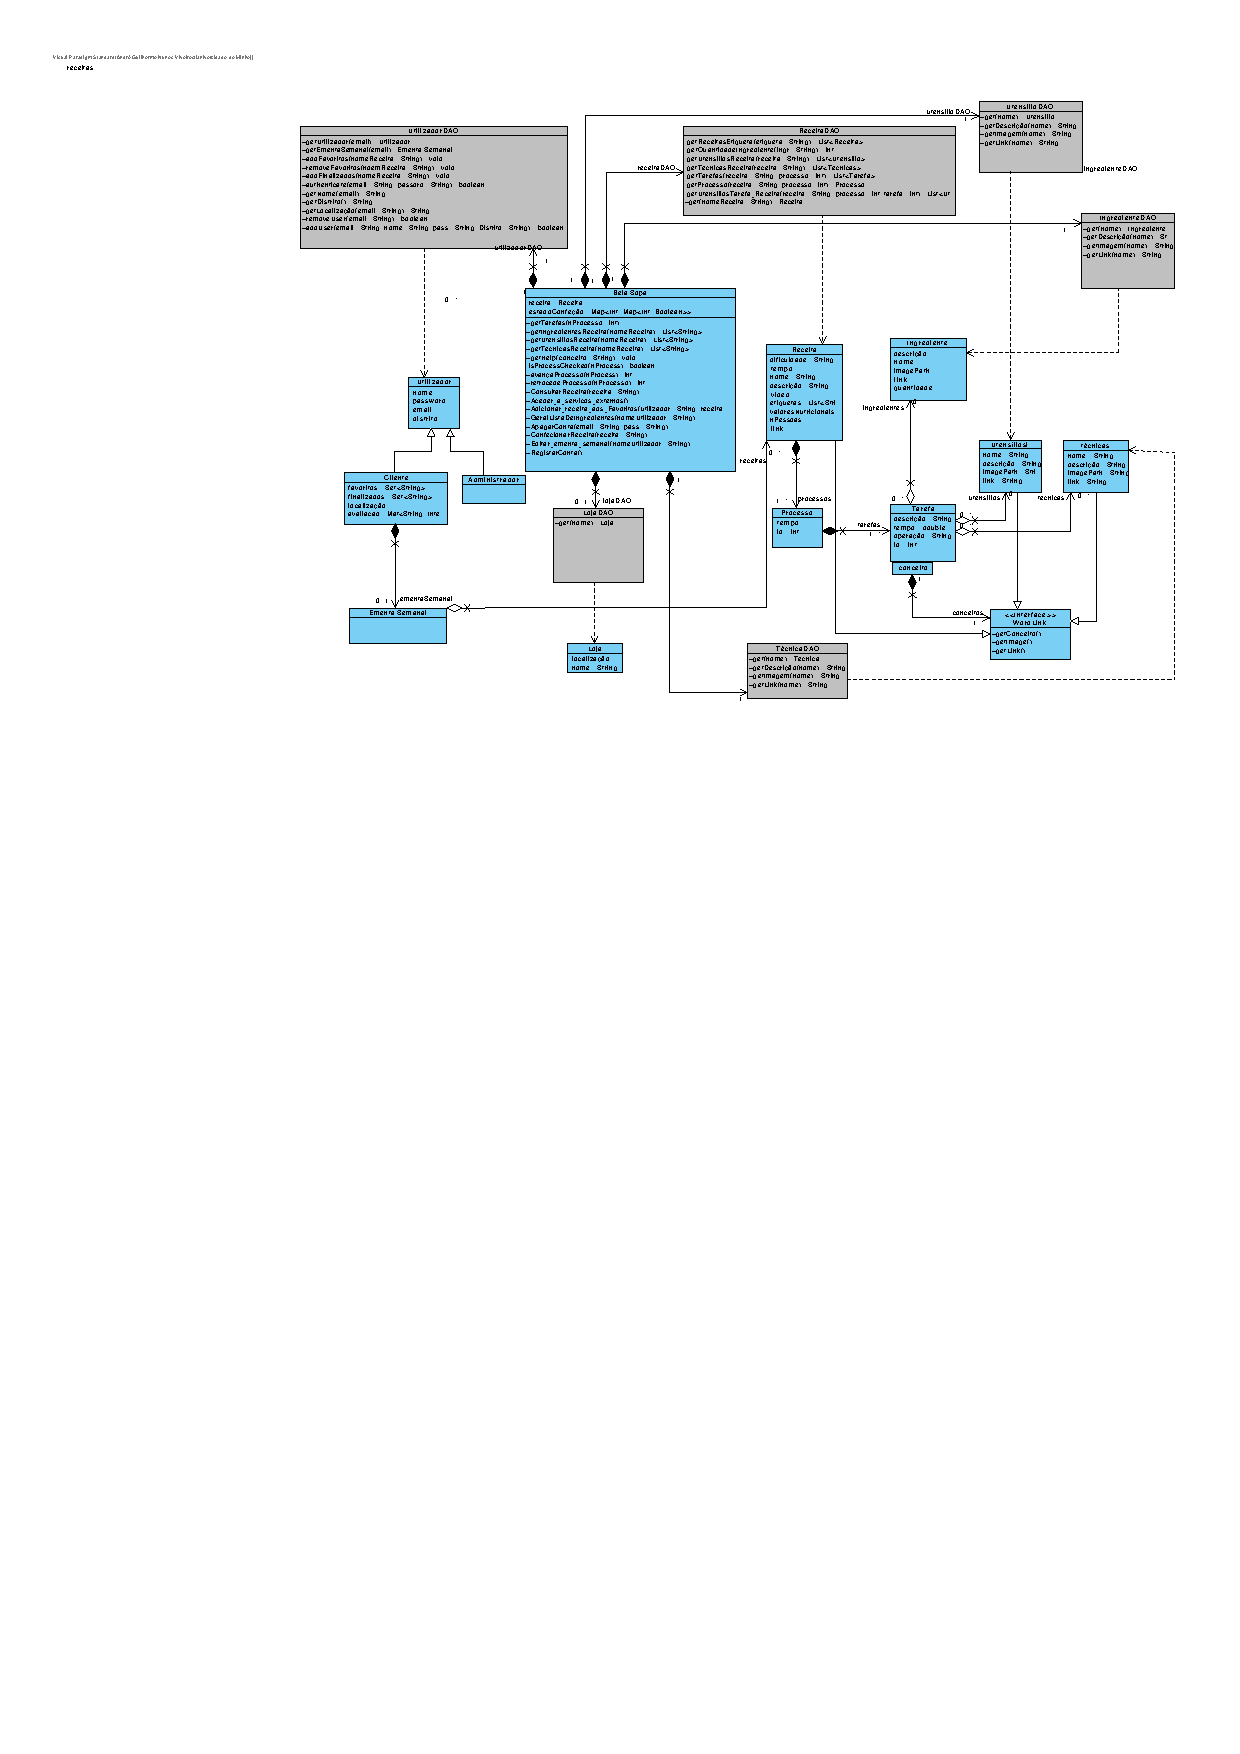
\includegraphics[width=\textwidth]{figures/09/Diagram_classe_com_DAO.pdf}
  \caption{Diagrama de classes para a camada de dados.}
\end{figure}

% ---------------------------------------------------------------------------- %

\subsection{Modelação concetual da base de dados}
\label{sec:sbd:concetual:ent-rel-atr}

Foram subentendidos no diagrama de classes apresentado anteriormente, todos as entidades a serem criadas tais como os seus respectivos atributos.
Dito isto foram estabelecidas as relações entre as entidades. Para uma compreensão mais legível das mesmas decidiu-se utilizar o modelo concetual apenas para realçar estas relações, o qual é apresentado na \reffig{fig:concetuallllll} e utiliza a notação Chen~\parencite{chen1976entity}.

\begin{figure}[ht]
  \centering
  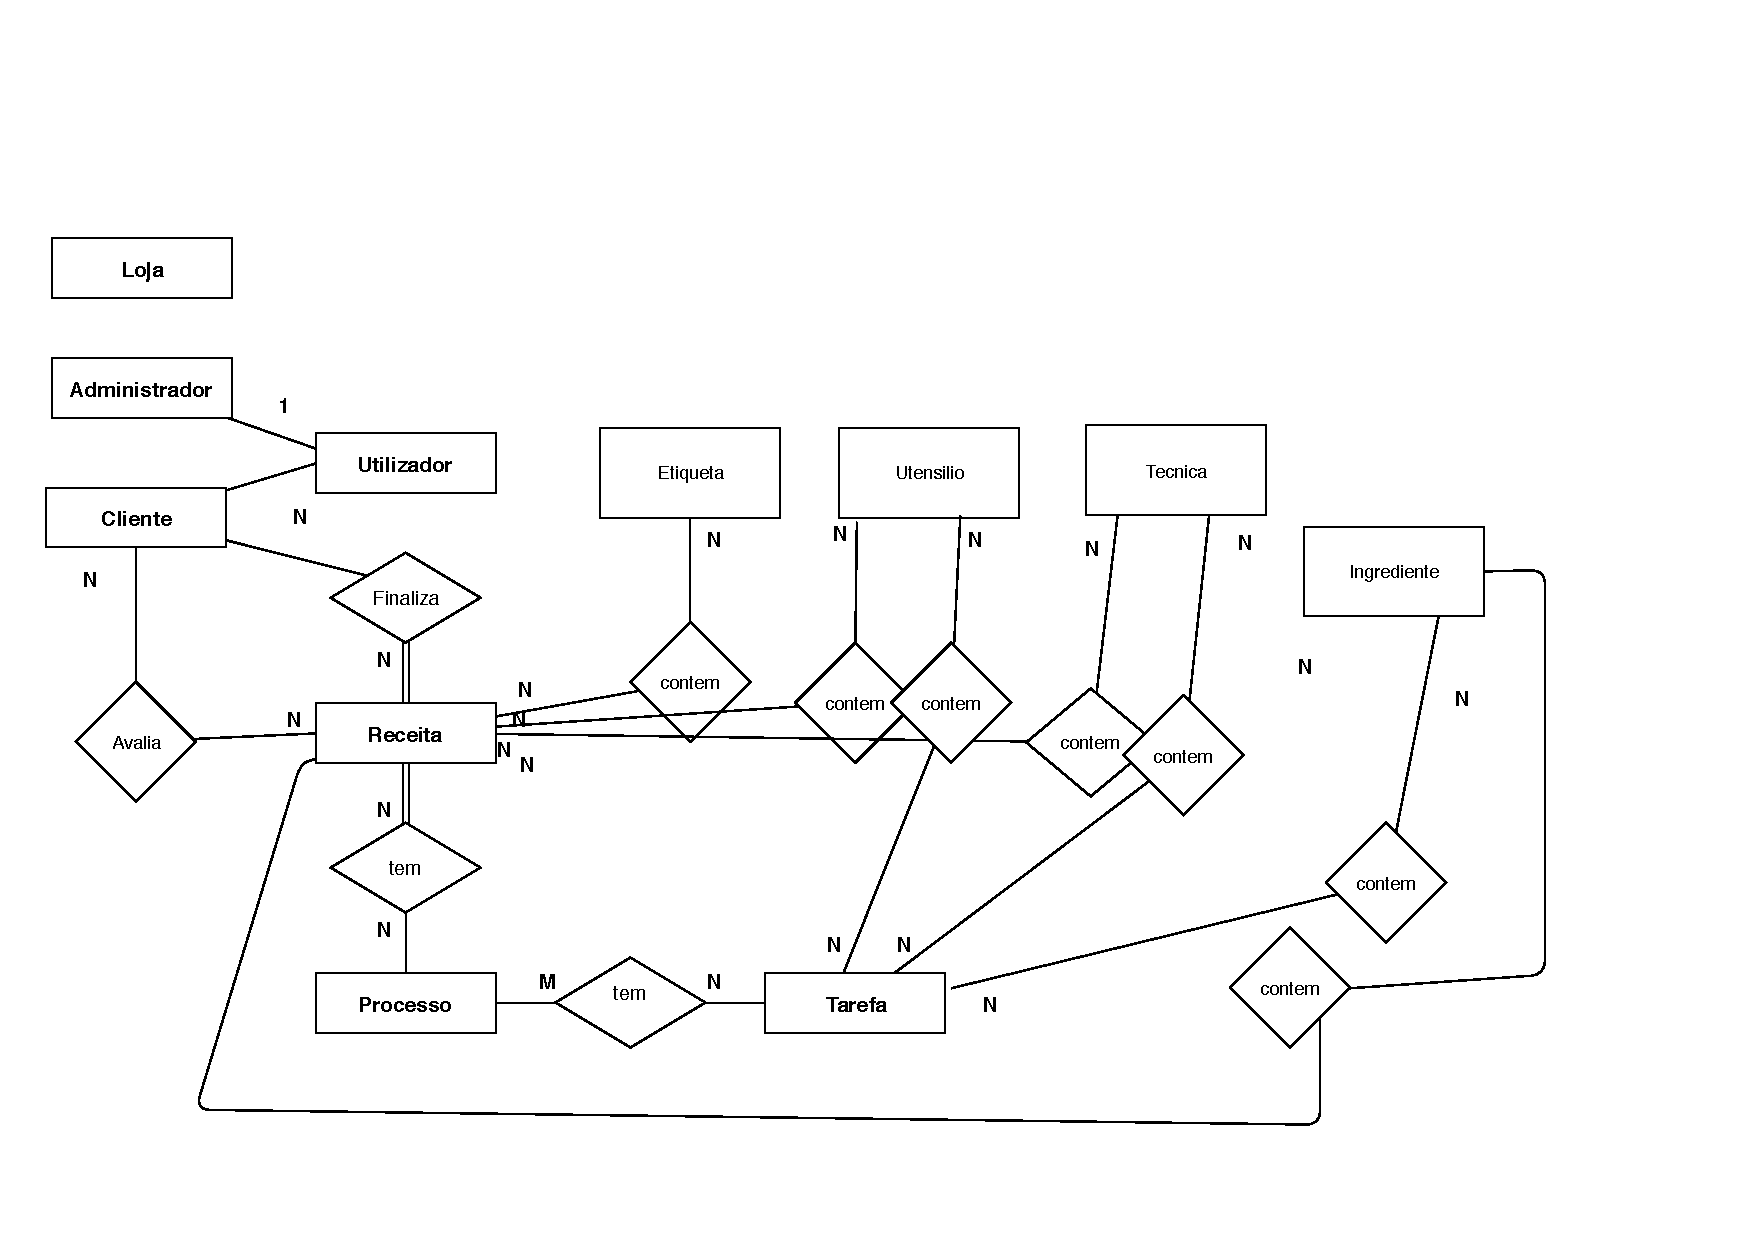
\includegraphics[width=\textwidth]{figures/09/sbd-concetual.pdf}
  \caption{Modelo concetual da base de dados.}
  \label{fig:concetuallllll}
\end{figure}

% ---------------------------------------------------------------------------- %

\subsection{Modelação lógica da base de dados}
\label{sec:sbd:logico}

Tendo as relações definidas elaborou-se o modelo lógico através do programa \emph{MySQL Workbench}\footnote{\url{https://www.mysql.com/products/workbench/}, acedido a 23 de maio de 2019}, o qual se apresenta na \reffig{fig:logicoooooooooo}.

\begin{figure}[ht]
  \centering
  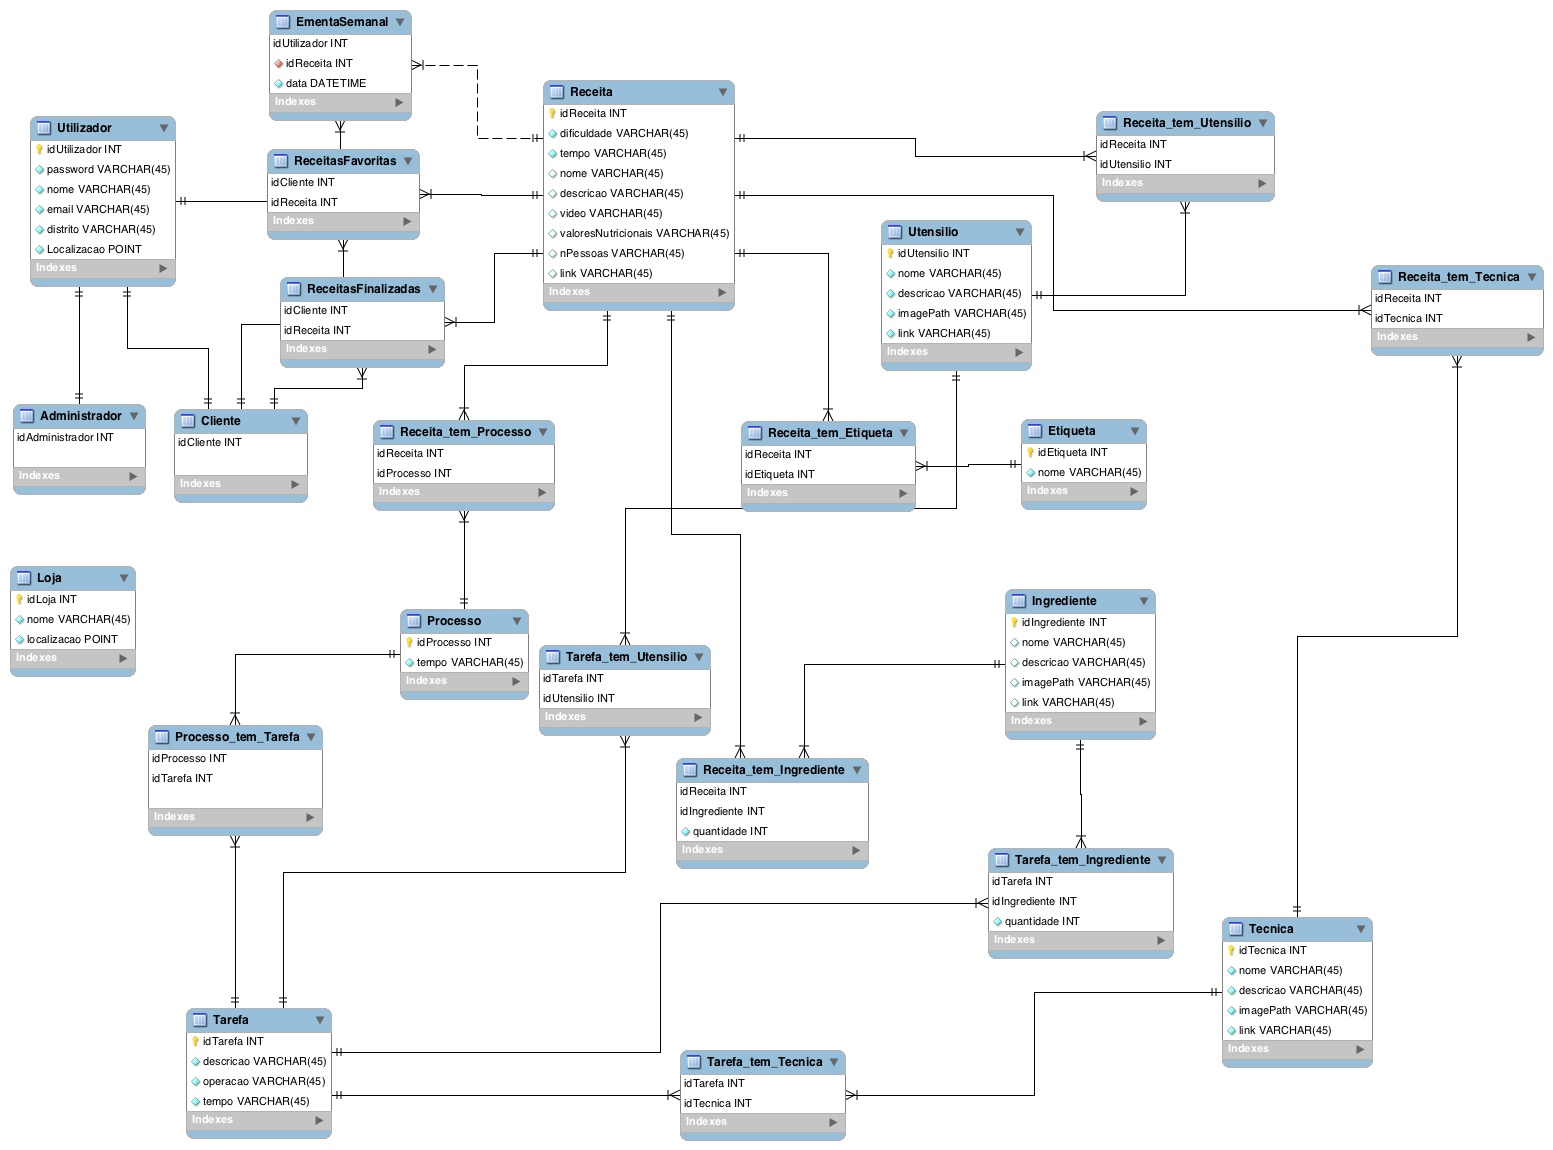
\includegraphics[width=\textwidth]{figures/09/sbd-logico.png}
  \caption{Modelo lógico da base de dados.}
  \label{fig:logicoooooooooo}
\end{figure}

% ---------------------------------------------------------------------------- %
%\subsubsection{Desenho do modelo}
%\label{sec:sbd:logico:desenho}
% ---------------------------------------------------------------------------- %
%\subsubsection{Validação do modelo}
%\label{sec:sbd:logico:validacao}
%\alberto{< através da normalização (até 3NF) >}
%\alberto{< com interrogações >}
%\alberto{< com transações >}
% ---------------------------------------------------------------------------- %
